% Fundamental theorem of calculus, pictorially: the net change of f over
% [t_0, t_3] (green arrows / blue "Net change") equals a sum of tangent
% (derivative) contributions at sample points xi_i (red).
% Source: book/tex/calculus/integrate.tex (§ Fundamental theorem of calculus).
\documentclass[border=2mm]{standalone}
\usepackage{tikz}
\begin{document}
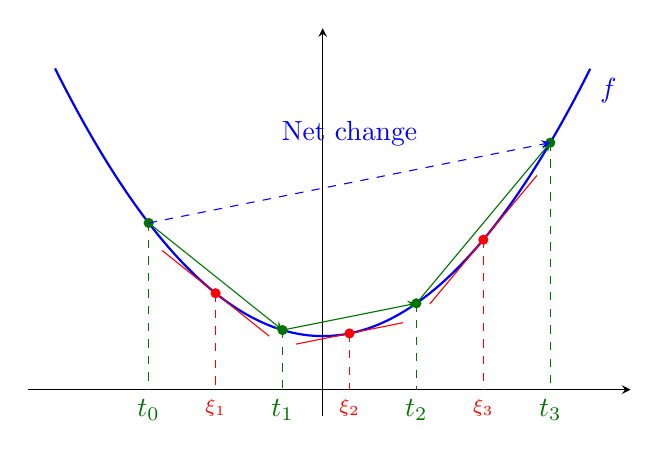
\begin{tikzpicture}[scale=1.7,
    dot/.style={circle,fill,inner sep=1.3pt},
    >=stealth]
  \draw[->] (-2.2,0)--(2.3,0);
  \draw[->] (0,-0.2)--(0,2.7);
  \draw[blue,thick,domain=-2:2,samples=100] plot (\x, {\x*\x/2+0.4});
  \node[blue,below right] at (2,2.4) {$f$};
  % sample points t_0..t_3 with green net-change arrows
  \foreach \x/\y in {-1.3/1.245, -0.3/0.445, 0.7/0.645, 1.7/1.845}
    \node[dot,green!45!black] at (\x,\y) {};
  \draw[green!45!black,->] (-1.3,1.245)--(-0.3,0.445);
  \draw[green!45!black,->] (-0.3,0.445)--(0.7,0.645);
  \draw[green!45!black,->] (0.7,0.645)--(1.7,1.845);
  % dashed green drop-lines and t labels
  \foreach \x/\lbl in {-1.3/{t_0}, -0.3/{t_1}, 0.7/{t_2}, 1.7/{t_3}} {
    \pgfmathsetmacro\y{\x*\x/2+0.4}
    \draw[green!45!black,dashed] (\x,\y)--(\x,0);
    \node[green!45!black,below] at (\x,0) {$\lbl$};
  }
  % red tangents at xi_1,xi_2,xi_3 = -0.8, 0.2, 1.2 (slope = xi)
  \foreach \m in {-0.8, 0.2, 1.2} {
    \pgfmathsetmacro\y{\m*\m/2+0.4}
    \node[dot,red] at (\m,\y) {};
    \draw[red] ({\m-0.4},{\y-0.4*\m})--({\m+0.4},{\y+0.4*\m});
    \draw[red,dashed] (\m,\y)--(\m,0);
  }
  \foreach \m/\lbl in {-0.8/{\xi_1}, 0.2/{\xi_2}, 1.2/{\xi_3}}
    \node[red,below,font=\scriptsize] at (\m,0) {$\lbl$};
  % net change
  \draw[blue,dashed,->] (-1.3,1.245)--(1.7,1.845);
  \node[blue,above] at (0.2,1.75) {Net change};
\end{tikzpicture}
\end{document}
